\documentclass{article}
\usepackage[margin=1in]{geometry}
\usepackage[T1]{fontenc}
\usepackage{csquotes}
\usepackage{url}
\usepackage{graphicx}
\usepackage{caption}
\usepackage{xcolor,colortbl}
\usepackage{textcomp} 
\usepackage{pythonhighlight}
\usepackage{enumitem}
\usepackage{float}
\usepackage{subfig}
\usepackage{hyperref}
\usepackage{indentfirst}
\renewcommand{\familydefault}{\sfdefault}

\newcommand{\mc}[2]{\multicolumn{#1}{c}{#2}}
\definecolor{Gray}{gray}{0.95}
\definecolor{LightCyan}{rgb}{0.88,1,1}

\newcolumntype{a}{>{\columncolor{Gray}}l}
\newcolumntype{b}{>{\columncolor{white}}c}

\graphicspath{{./img/}}


% Listings
\definecolor{pblue}{rgb}{0.13,0.13,1}
\definecolor{pgreen}{rgb}{0,0.5,0}
\definecolor{pred}{rgb}{0.9,0,0}
\definecolor{pgrey}{rgb}{0.46,0.45,0.48}

\lstset{language=Java,
  showspaces=false,
  showtabs=false,
  breaklines=true,
  showstringspaces=false,
  breakatwhitespace=true,
  commentstyle=\color{pgreen},
  keywordstyle=\color{pblue},
  stringstyle=\color{pred},
  basicstyle=\ttfamily
}


\definecolor{codegray}{gray}{0.95}
\definecolor{commentgray}{gray}{0.35}

\makeatletter

\begin{document}

\title{SER 222: ADJ Problem 3}
\author{Claudio Rodriguez Rodriguez}
\maketitle

% task_struct - from <linux/sched.h> <-- defined here

% for_each_process - from <linux/sched/signal.h> <-- defined here (MACRO)

% list_for_each - from #include <linux/list.h> <-- defined here (MACRO)
% list_entry - from #include <linux/list.h>  <-- defined here (MACRO)
% list_head - from #include <linux/list.h>

% module_param - from #include <linux/moduleparam.h> <-- defined here (MACRO)
% MODULE_PARM_DESC - from #include <linux/moduleparam.h> <-- defined here (MACRO)

% printk - from <linux/kernel.h> 
% defined in #include <linux/printk.h>
% function

% print_header
% print_row
% init_rodriguez_rodriguez_lkm_module
% exit_rodriguez_rodriguez_lkm_module

\section{Using Graphs for Contact Tracing}

\subsection{Problem}

\textit{Develop a system to perform contact tracing to notify individuals who may have been exposed to an infectious disease.}

\subsection{Analysis}

We need to contact individuals in `close contact` with people or venues compromised by disease. The project needs to produce results quickly and notify people who might be false positive. The algorithm also needs to be able to throttle notification systems considering that some notifications are more important than others. Multiple message avenues are preferable, but they might have different arrival dates. 

\subsubsection{Assumptions}

We are given a list of people that have been in the same place at the same time. 

We receive a list of people who have been in the same place simultaneously. Therefore, our system will need to use a person classified as `infected.` Using `infected` people, our approach must find close contacts inside that list of people. We assume that our system will receive infected people from whoever is using it. We assume people are tagged with a trace of geodetic datum and timestamps in the specific venue.

We assume we have various notification systems at our disposal and that all of those might fail. We also assume that the notification systems are not reliable. 

\subsubsection{Metrics}

From the problem, we observe two problems with different set of metrics:

\paragraph{Finding Close Contacts (F)}

\begin{itemize}
  \item FM1: The efficiency of the algorithm. We use the number of comparisons in the algorithm as a cost metric to measure the computational time needed for a particular design.
  \item FM2: Memory efficiency of the algorithm. We use the amount of memory needed to run the algorithm as a cost metric in the form of variables required. 
  \item FM1: The algorithm returns a list of close contacts. We use the number of close contacts as a cost metric to measure the number of close contacts returned.
\end{itemize}

\paragraph{Notifying Close Contacts (N)}

\begin{itemize}
  \item NM1: The efficiency of the algorithm. We use the number of comparisons in the algorithm as a cost metric to measure the computational time needed for a particular design. 
  \item NM2: The ability of the algorithm to select only the highest priority contacts.
\end{itemize}

\subsection{Design}

The definition of the problem and the assumptions leave a vast amount of leeway to design the problem. The goal is to find and notify close contacts as fast as possible and via multiple methods. But this also means that a person needs to have a "root" of the notification. If a person appears as infected without any close contact, we declare the event as this person and timestamp. This tag allows us to mark close contacts and notify them based on this contact. But we can also handle the scenario if the `close contact` is in contact with a new "root" case.

\paragraph{Finding Close Contacts}

The Selected Solution for Finding Close Contacts would look like an Undirected Graph using Adjacency List that utilizes Breadth-First Search to retrieve all Neighbor Contacts from a specific contact. An example of how a graph would look like on a Venue is presented in Figure~\ref{fig:closeContacts}. We would insert a new level into the graph using the euclidean distance between 2 contacts' geolocation. This property would allow us to stack each graph level as the closest contact to a certain distance. 

To find a close connection or an `infected person` in the Graph, we would traverse it using DFS, but once we find it, we would retrieve the N number of contacts close to that Vertex using BFS. 

Each person might appear more than once in the Graph, and thus we use an ID to identify them. When we search the Graph, we add the results to a Set of Results so that if it appears more than once during the timeframe, our Set automatically removes the duplicate.

\begin{figure}[h!]
  \centering
  \captionsetup{justification=centering}
  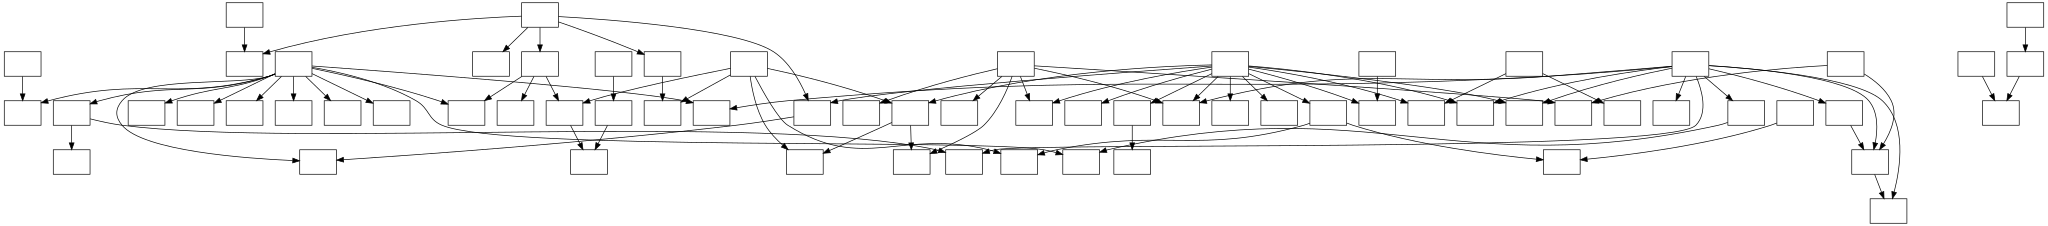
\includegraphics[width=0.5\textwidth]{graph.png}
  \caption{
    Example structure of Close Contacts
  }%
  \label{fig:closeContacts}%
\end{figure}

\paragraph{Notifying Close Contacts}

To Notify Close Contacts, we use a Priority Queue where we use the min distance together with a counter (to maintain key uniqueness) as the priority. Therefore, the shortest distance would receive the highest priority. We also use the priority as a metric, and the higher priorities would go to multiple systems that handle emails, calls, and SMS messages. 

\subsection{Justification}

\subsubsection{Finding Close Contacts}

\paragraph{FM1}

The algorithm will check for $O(N)$ neighbor contacts when using the adjacency list compared to the $O(V)$ time complexity of the adjacency matrix. Using BFS an structuring the nodes using distance would also help in only searching the closest neighbors so that we can respect the Big-Oh Complexity.

\paragraph{FM2}

The algorithm will use $O(V + E)$ space complexity compared to $O(V^2)$ space complexity of the adjacency matrix.

\paragraph{FM3}

Both BFS and DFS would work to find close contacts, but due to the nature of the problem, we would save some checks using BFS. However, this disadvantage does not mean that DFS is not a viable solution. The problem is structured to use BFS, and similarly, it can be structured to use DFS. 

\subsubsection{Notifying Close Contacts}

\paragraph{NM1}

A priority Queue means we have $O(log(n))$ insertion times and $O(1)$ removal times using an underlying Heap Data Structure. We wouldn't be using the structure for searching.

\paragraph{NM2}

A Priority Queue would allow the algorithm to prioritize the notifications based on the distance. The prioritization would enable us to send the notifications to the closest contacts first. But, more importantly, we can throttle our communications depending on the availability of the external services.

\subsection{Alternative Design}

An alternative design for the Finding Contacts problem would be defining what "close contact" means from the beginning. Then we could group contacts in a single node. Then, our search would traverse a graph and find the person inside a list of persons inside the node. However, this design would not take advantage of the graph properties, making it less likely to be able to meet the criteria of the other metrics.


\end{document}
